\documentclass{article}

% if you need to pass options to natbib, use, e.g.:
%     \PassOptionsToPackage{numbers, compress}{natbib}
% before loading neurips_2020

% ready for submission
% \usepackage{neurips_2020}

% to compile a preprint version, e.g., for submission to arXiv, add add the
% [preprint] option:
%     \usepackage[preprint]{neurips_2020}

% to compile a camera-ready version, add the [final] option, e.g.:
%     \usepackage[final]{neurips_2020}

% to avoid loading the natbib package, add option nonatbib:
\usepackage[nonatbib, final]{stat520a}
\usepackage[autonum]{../macros}
\usepackage{natbib}
\setcitestyle{brackets=round}

\usepackage[utf8]{inputenc} % allow utf-8 input
\usepackage[T1]{fontenc}    % use 8-bit T1 fonts
\usepackage{hyperref}       % hyperlinks
\usepackage{url}            % simple URL typesetting
\usepackage{booktabs}       % professional-quality tables
\usepackage{amsfonts}       % blackboard math symbols
\usepackage{nicefrac}       % compact symbols for 1/2, etc.
\usepackage{microtype}      % microtypography
\usepackage{lmodern}

\newcommand{\alr}{\mathrm{alr}}

\title{A general-purpose Bayesian model for estimating election results in Mexico}

% The \author macro works with any number of authors. There are two commands
% used to separate the names and addresses of multiple authors: \And and \AND.
%
% Using \And between authors leaves it to LaTeX to determine where to break the
% lines. Using \AND forces a line break at that point. So, if LaTeX puts 3 of 4
% authors names on the first line, and the last on the second line, try using
% \AND instead of \And before the third author name.

\author{%
  Gian Carlo Di-Luvi \\
  %\thanks{Use footnote for providing further information
  %  about author (webpage, alternative address)---\emph{not} for acknowledging
  %  funding agencies.} \\
  Department of Statistics\\
  University of British Columbia \\
  \texttt{gian.diluvi@stat.ubc.ca}
  % examples of more authors
  % \And
  % Coauthor \\
  % Affiliation \\
  % Address \\
  % \texttt{email} \\
  % \AND
  % Coauthor \\
  % Affiliation \\
  % Address \\
  % \texttt{email} \\
  % \And
  % Coauthor \\
  % Affiliation \\
  % Address \\
  % \texttt{email} \\
  % \And
  % Coauthor \\
  % Affiliation \\
  % Address \\
  % \texttt{email} \\
}

\begin{document}

\maketitle

\begin{abstract}
  In Mexico, estimating the results of the election the day it takes place is a tradition that gives certainty to the electoral process. For this purpose, electoral authorities organize a quick count, in which a random sample of polling stations is used to estimate the results of the election. Multiple Bayesian models have been used in Mexican quick counts since 2006. However, these models assume that candidates are independent, which has a negative impact on model accuracy. In this work, we propose a general-purpose model that takes care of these issues by forcing the proportions of votes to reside in the probabilistic simplex and assuming an arbitrary covariance structure. We discuss uninformative prior distributions for both the proportions in the simplex and the covariance matrix and compare the model with one of the models used in the 2018 Mexican presidential election.
\end{abstract}



\section{Introduction} \label{sec:intro}


In Mexico, presidential and gubernatorial elections take place every six years. Mexico has a multi-party electoral system where the candidate that receives the largest amount of votes wins the election. Because election results take a week to be certified, in recent years there has been a widespread effort by government authorities to determine the winner of each election the day it takes place. For this purpose, a sample of polling stations is usually selected before the election and statistical estimates based on those polling stations are computed as the results become available on election day---a process called a \textit{quick count} \citep{carrera2019}.
\\



Multiple Bayesian models have been used in Mexico's quick counts. \citet{mendoza-nieto2016} proposed a simple Bayesian model with a tractable posterior to estimate the proportion of votes in favor of each candidate in the 2006 and 2012 elections. \citet{cerrillo2019} used the same model in the 2016 elections of Veracruz, a state in the east cost of Mexico. \citet{diluvi2018} modified that same model and used it to predict the results of the 2018 election. \citet{anzarut2018} proposed a Bayesian multilevel regression model and used it in the 2018 election as well.
\\




On election day, data from the polling stations arrive as field personnel finish counting the votes: every 5 minutes, new data are supplied and models have to be retrained. Thus, models should be rich enough to do accurate inference with small sample sizes while allowing for fast online inference. The model in \citep{anzarut2018} accounts for data missing not at random but is computationally expensive---for the presidential election, it took well over 5 minutes to run even when parallelising over 48 CPU cores. On the other hand, although the model proposed by \citep{mendoza-nieto2016} is easy to train, they rely on a tractable posterior distribution that severly overestimates the voter turnout. \citet{diluvi2018} modified the prior distribution to remedy this, but they did not account for the corresponding change in the posterior.
\\

One of the main issues with previous models is that the candidates are treated independently. In this work, we address this issue by forcing the proportions of votes to reside in the probabilistic simplex $\Delta^{J-1}$. Furthermore, by working with a multivariate joint model for all candidates, we design models with arbitrary covariance structures. Finally, we implement an MCMC sampling scheme in \textsc{Stan} \citet{rstan} to fit all these models.
\\

In Section \ref{sec:background}, we present the original model in \citet{mendoza-nieto2016}, as well as the modifications by \citet{diluvi2018}. In Section \ref{sec:model}, we show how to modify the model to properly account for both the proportions of votes and an arbitrary covariance structure. We implement the original models and two new models in Section \ref{sec:experiments}, and conclude the paper in Section \ref{sec:conclusion}.


\section{Background} \label{sec:background}


Quick counts are organized by the Mexican Electoral Institute but carried out by a committee of statisticians. Each member of the committe proposes and implements a different model. On election day, each model is trained every 5 minutes when new information becomes available, and the results from all models are combined into a single interval per candidate. When the committee decides that the sample is sufficiently large, the final combined intervals are reported to the government authorities. \\

To determine the sample of polling stations, a stratified sampling design is developed by the committee. The observational unit corresponds to the polling station and the strata---which vary from election to election---are defined based on geographical variables. Suppose that the population of polling stations is divided into $N$ strata, and that stratum $i$ has $K_i$ polling stations. Although the number of voters is unknown before the election, the number of \textit{registered voters} per polling station is known in advance. Let $n_i^k$ be the number of registered voters in polling station $k$ of stratum $i$. \\

The observables in the model correspond to the number of votes, which for each candidate $j$, stratum $i$, and polling station $k$ we denote by $X_{ij}^k$. The latent variables correspond to the proportion of votes, which for candidate $j$ and in stratum $i$ are denoted by $\theta_{ij}$. In these definitions, we use the term candidate loosely to refer to actual candidates as well as the set of null votes and the set of votes that were not cast. Note that we assume that all polling stations within a stratum have the same proportion of votes per candidate, i.e.
\[
\theta_{ij} = \frac{\sum_{k=1}^{K_i} X_{ij}^k}{\sum_{k=1}^{K_i} n_{i}^k}
\]
does not depend on $k$.\footnote{It is possible to assume that the proportions of votes vary by polling station, for example using Dirichlet processes \citep[see][]{lo1984class, nieto2018}, but learning the parameters becomes computationally expensive.} The national proportion of votes in favor of candidate $j$ is then
\[
  \theta_j = \frac{1}{n} \sum_{i=1}^N n_i \theta_{ij}, \label{eq:thetaj}
\]
where $n = \sum_{i=1}^N n_i$ is the total number of nation-wide registered voters. Observe that $\theta_j$ refers to the proportion of votes out of registered voters, rather than out of cast votes. We thus define, for each candidate $j$, the effective proportion of votes as
\[
  \lambda_j = \frac{\theta_j}{\sum_{r = 1}^{J-1} \theta_r},  \label{eq:lambdaj}
\]
where the sum is over all proper candidates (i.e. excluding $\theta_J$, which corresponds to uncast ballots). \\



\citet{mendoza-nieto2016} propose modeling the number of votes in polling station $k$ of stratum $i$ and in favor of candidate $j$ via
\[
  X_{ij}^k \sim \distNorm \left( n_i^k \theta_{ij}, \frac{\tau_{ij}}{n_i^k} \right), \label{eq:original_likelihood}
\]
where $\tau_{ij}$ is a precision parameter.\footnote{Although $\frac{\tau_{ij}}{n_i^k}$ corresponds to the variance of the distribution.} The number of votes are assumed to be independent between candidates, which is inaccurate because, at each polling station, the total votes should add up to the known number of registered voters, $n_i^k$. \citet{mendoza-nieto2016} acknowledge this issue but argue that including a correlation structure, although correct in theory, produces small improvements in accuracy. \\


Because the quick counts are organized by governmental authorities, prior distributions should assign the same likelihood of winning to each candidate. \citet{mendoza-nieto2016} use uniform distributions for $\theta_{ij}$ and an independent improper prior for $\tau_{ij}$. With these, the posterior distribution after observing the information from $c_i$ polling stations in stratum $i$ has a closed form, namely
\[ \label{eq:original_posterior}
  p(\theta_{ij}, \tau_{ij} \given X_{ij}^1, ..., X_{ij}^{c_i}) \propto \; &\distNorm \left(\theta_{ij} \; \Bigg\vert \; \frac{ \sum_{k=1}^{c_i} x_{ij}^{k} }{ \sum_{k=1}^{c_i} n_{i}^{k} }, \; \tau_{ij} \sum_{k=1}^{c_i} n_{i}^{k}  \right) \, \mathds{1}(0 < \theta_{ij} < 1) \\
    &\times \distGamma \left( \tau_{ij} \; \Bigg\vert \; \frac{c_{i} - 1}{2}, \; \frac{1}{2} \left\{ \sum_{k=1}^{c_i} \frac{ (x_{ij}^{k})^2 }{ n_{i}^{k} } - \frac{ \left( \sum_{k=1}^{c_i} x_{ij}^{k} \right)^2 }{ \sum_{k=1}^{c_i} n_{i}^{k} } \right\} \right).
\]
Sampling from Eqn. \refeq{eq:original_posterior} can be done expeditiously for each stratum---there is no need to run an MCMC scheme. Samples from all strata are then combined via Eqns. \refeq{eq:thetaj} and \refeq{eq:lambdaj} to obtain the national estimates for each candidate. \\

Because data arrive as field officers finish counting the votes, oftentimes entire strata in the sample have no information available. Notice that Eqn. \refeq{eq:original_posterior} requires $c_i >2$, i.e. information from at least two polling stations. In those strata, \citet{mendoza-nieto2016} sample from the prior distribution---which is the probability distribution that describes the uncertainty in the latent variables. However, because all candidates are assumed independent and $(\theta_{i1}, ..., \theta_{iJ})^\top$ is not constrained to add up to 1, it is possible that the estimated voter turnout, defined as
\[
  \rho = \sum_{j=1}^{J-1} \theta_j,
\]
exceeds 100\% in some strata---thereby causing the aggregated national average to be overestimated. \\

To remedy this, \citet{diluvi2018} proposed new prior distributions for $\theta_{ij}$---namely, Beta distributions with a mean equal to the historic voter turnout divided by the number of proper candidates. Although this seemingly takes care of the issue in practice, it does not technically resolve it because it fails to acknowledge that the proportion of votes, as a vector, lives in the probabilistic simplex. Furthermore, \citet{diluvi2018} only use the modified prior when no information is available from a given stratum. If information is available, samples are obtained from the tractable posterior, Eqn. \refeq{eq:original_posterior}, which does not correspond to the correct posterior associated with the modified prior distributions.



\section{Modeling proportions in the simplex} \label{sec:model}


To design a Bayesian model that correctly addresses the estimation of voter turnout, we first write the likelihood of votes in each stratum in Eqn. \refeq{eq:original_likelihood} as a multivariate Normal distribution. Specifically, letting $X_i^k = (X_{i1}^k,..., X_{iJ}^k)^\top$ and $\theta_i = (\theta_{i1}, ..., \theta_{iJ})^\top$, Eqn. \refeq{eq:original_likelihood} is equivalent to
\[
  X_i^k \sim \distNorm_J \left( n_i^k \theta_i, \Sigma_i^k \right),
\]
where $\Sigma_i^k = \diag(\tau_{i1}, ..., \tau_{iJ}) / n_i^k$. Observe that the number of votes is discrete. A multinomial distribution would be technically better suited to model $X_i^k$, and it would also ensure that the votes add up to the number of registered voters. However, it would also limit the flexibility of the model because, while possible to control the mean, the correlation structure of a multinomial distribution is determined by the means of each marginal Binomial distribution.
\\


Given that the number of registered voters is usually high,\footnote{In 2018, the average $n_i^k$ was 550.} using a Normal approximation to a Binomial distribution is well justified. Furthermore, by adding variance parameters independent of the mean, \citet{mendoza-nieto2016, diluvi2018} are able to model more complex variability structures. This approach has two shortcomings. The first is that it assumes that the vector $\theta_i$ lives in $[0, 1]^J$, when in reality $\theta_i$ lives in the probabilistic simplex $\Delta^{J-1} = \{ \theta \in \reals^J \given \theta_j > 0, \sum_{j=1}^J \theta_j = 1 \}$. This is the cause of the voter turnout overestimation. The second issue is that it assumes a trivial covariance structure.
\\


We overcome these issues by \textit{(i)} forcing $\theta_i \in \Delta^{J-1}$ and \textit{(ii)} letting $\Sigma_i^k$ be an arbitrary covariance matrix. The only additional requirements to fit this more complex model are to carefully design a prior distribution for $\theta_i$ in $\Delta^{J-1}$ and a prior distribution for $\Sigma_i^k$ in the space of covariance matrices.


\subsection{Prior distributions}


To design a prior distribution for $\theta_i$, observe that the dimension of $\Delta^{J-1}$ is $J-1$; indeed, $\Delta^{J-1}$ and $\reals^{J-1}$ are isomorphic. Consider the map $\mcA: \Delta^{J-1} \to \reals^{J-1}$ given by
\[
  \mcA (\theta_1, ..., \theta_J) = \left( \log \frac{\theta_1}{\theta_J}, ..., \log \frac{\theta_{J-1}}{\theta_J} \right)^\top.
\]
$\mcA$ is known as the \textit{additive log-ratio} \citep{aitchison1982}, and its inverse is given by
\[
  \mcA^{-1} (x_1, ..., x_{J-1}) = \left( \frac{\exp(x_1)}{1 + \sum_{i=1}^{J-1} \exp(x_i)}, ..., \frac{\exp(x_{J-1})}{1 + \sum_{i=1}^{J-1} \exp(x_i)}, \frac{1}{1 + \sum_{i=1}^{J-1} \exp(x_i)} \right)^\top.
\]
The additive log-ratio transform is closely related to the center log-ratio transform, whose inverse is the popular softmax function. However, we choose to work with $\mcA$ because it is easier to interpret, and thus to define a prior on the transformed values. \\

In the transformed space $\reals^{J-1}$, the coordinate $j$th corresponds, up to additive constants, to the log of the proportion of votes in favor of candidate $j$, for $j=1, ..., J-1$. We assume that the $J$th candidate corresponds to the set of uncast ballots, which is of less interest. For the rest of the candidates, we define a Normal prior and choose the mean so that, when mapped back to $\Delta^{J-1}$ via $\mcA^{-1}$, it coincides with that of \citet{diluvi2018}: the historic voter turnout divided by the number of candidates. A dependence structure is introduced when mapping back into the simplex via $\mcA^{-1}$.
\\


Perhaps the best known distribution in the space of covariance matrices is the Wishart distribution, which is the multivariate generalization of the Gamma distribution. The Wishart distribution was popularized because it is the conjugate prior for the covariance matrix of Normally-distributed populations. However, the purpose of the prior being to quantify the prior knowledge of the parameters, we consider it best to choose a distribution that reflects the vague knowledge we have of the correlation structure between candidates.
\\

For this purpose, we decompose $\Sigma_i^k = \diag(\sigma_1, ..., \sigma_J) P \diag(\sigma_1, ..., \sigma_J) / n_i^k$, where $P$ is the correlation matrix and $\sigma_j$ is the variance of each candidate. \citet{lewandowski2009} propose a method to generate correlation matrices uniformly over the space of all correlation matrices. We use their method, through its \textsc{Stan} implementation, and couple it with uninformative priors for the variances. This results in an uninformative prior for the covariance matrix.
\\

%The new model can be summarised as
%\[
%  X_i^k &\sim \distNorm_J \left( n_i^k \theta_i, \Sigma_i^k \right), \quad k=1, ..., K_i, \; i=1, ..., N, \\
%  \theta_i &= \mcA^{-1}(X), \; X \sim \distNorm_{J-1} \\
%  \Sigma_i^k &= \frac{1}{n_i^k} \diag(\sigma_1, ..., \sigma_J) P \diag(\sigma_1, ..., \sigma_J), \quad P \sim \distUnif, \sigma_j^2 \sim \distUnif.
%\]



\section{Experiments} \label{sec:experiments}


We study the results of the 2018 Presidential election and compare four different models:
\benum
  \item The model used by \citet{diluvi2018} in the 2018 elections, which contains modified Beta priors but samples from the original posterior in \citet{mendoza-nieto2016};
  \item that same model but now sampling from the correct posterior via MCMC;
  \item the model proposed in Section \ref{sec:model} but assuming a trivial correlation structure, i.e., $P = I_J$;
  \item and the same new model but with an arbitrary covariance structure and the uninformative prior on the covariance matrix.
\eenum
In the third model, the proportions of votes are forced to live in the probabilistic simplex but the correlation structure assumes a simple form, which results in faster sampling. \\

For model 1, we generate 10,000 observations from the posterior distribution of $(\lambda_1, ..., \lambda_5)$ and $\rho$. For models 2 and 3, we generate 1,000 observations, and for model 4 only 500 due to the excessive computing time required to fit the model. Code can be found on \href{https://github.com/GiankDiluvi/bayes-quick-counts-2020}{\url{https://github.com/GiankDiluvi/bayes-quick-counts-2020}}. \\


We focus our attention on the winner of the election, AMLO. Figure \ref{fig:amlo} shows the posterior distribution of the proportion of votes in favor of him at 22:30pm---the time at which the quick counts committee decided to make the results public. Notably, models 2 and 3 have a smaller variance than models 1 and 4. Furthermore, model 1 underestimates the proportion of votes, possibly because strata with few polling stations have a bigger impact than on the other models. However, as seen in the right panel of Figure \ref{fig:amlo}, all four models close in on the true value at approximately the same rate. \\


\begin{figure}[h]
  \centering
  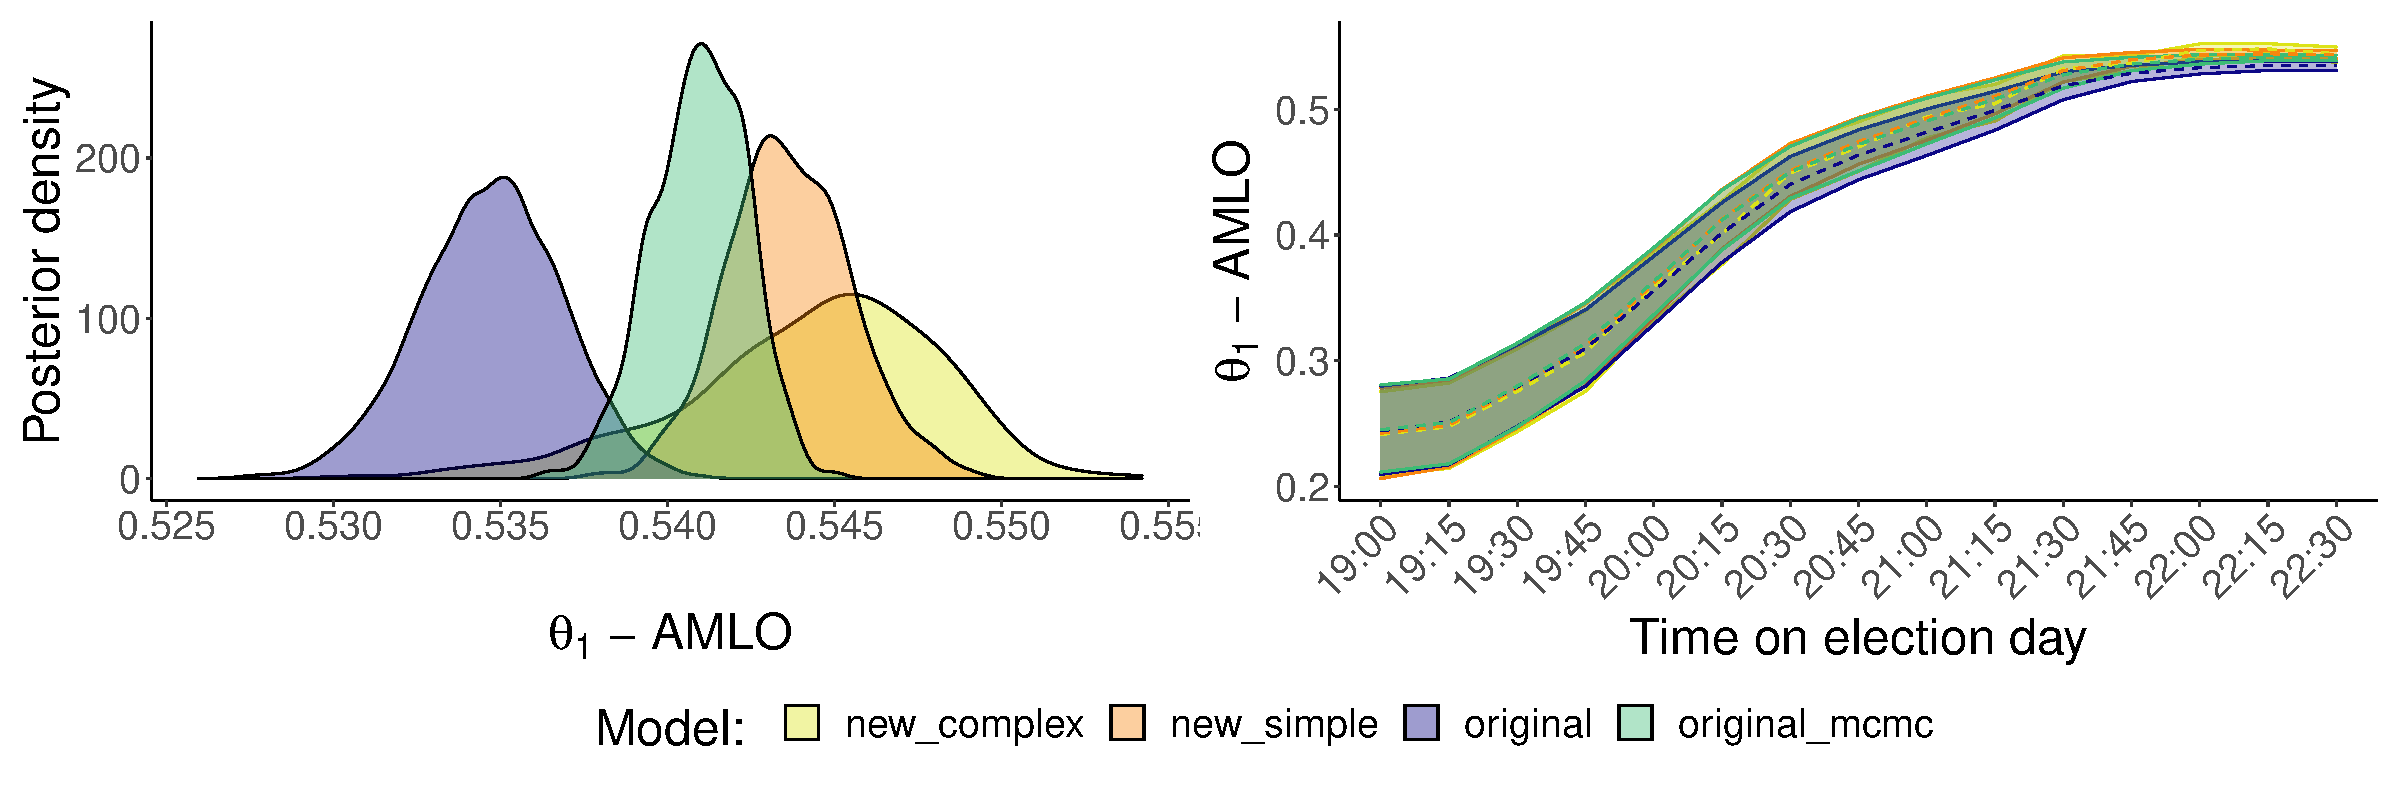
\includegraphics[width=\textwidth]{../fig/amlo.pdf}
  \caption{The left panel shows the posterior distribution of the proportion of votes in favor of AMLO at 22:30pm, with models by color. The right panel shows the mean and 0.025 and 0.975 quantiles (giving a 95\% posterior credible interval) for different times. \texttt{new\_complex} refers to model 4, \texttt{new\_simple} to model 3, \texttt{original} to model 1, and \texttt{original\_mcmc} to model 2.}
  \label{fig:amlo}
\end{figure}


The real advantage of the models in which the proportion of votes is forced to be an element of $\Delta^{J-1}$ is in the estimation of the voter turnout, which can be seen in Figure \ref{fig:part}. Inspecting the right panel, we see that the new model (both with and without a complex covariance structure) produces smaller estimates, whereas the original model in both its versions overestimates the turnout. Notably, the modification by \citet{diluvi2018} does a good job at reducing the overestimation, but the new model completely addresses this issue. This is even more clear in the right panel, where we see that, during the early hours of election day---when multiple strata are missing and so samples from the prior are generated---the new model produces considerably shorter credible intervals. \\


\begin{figure}[h]
  \centering
  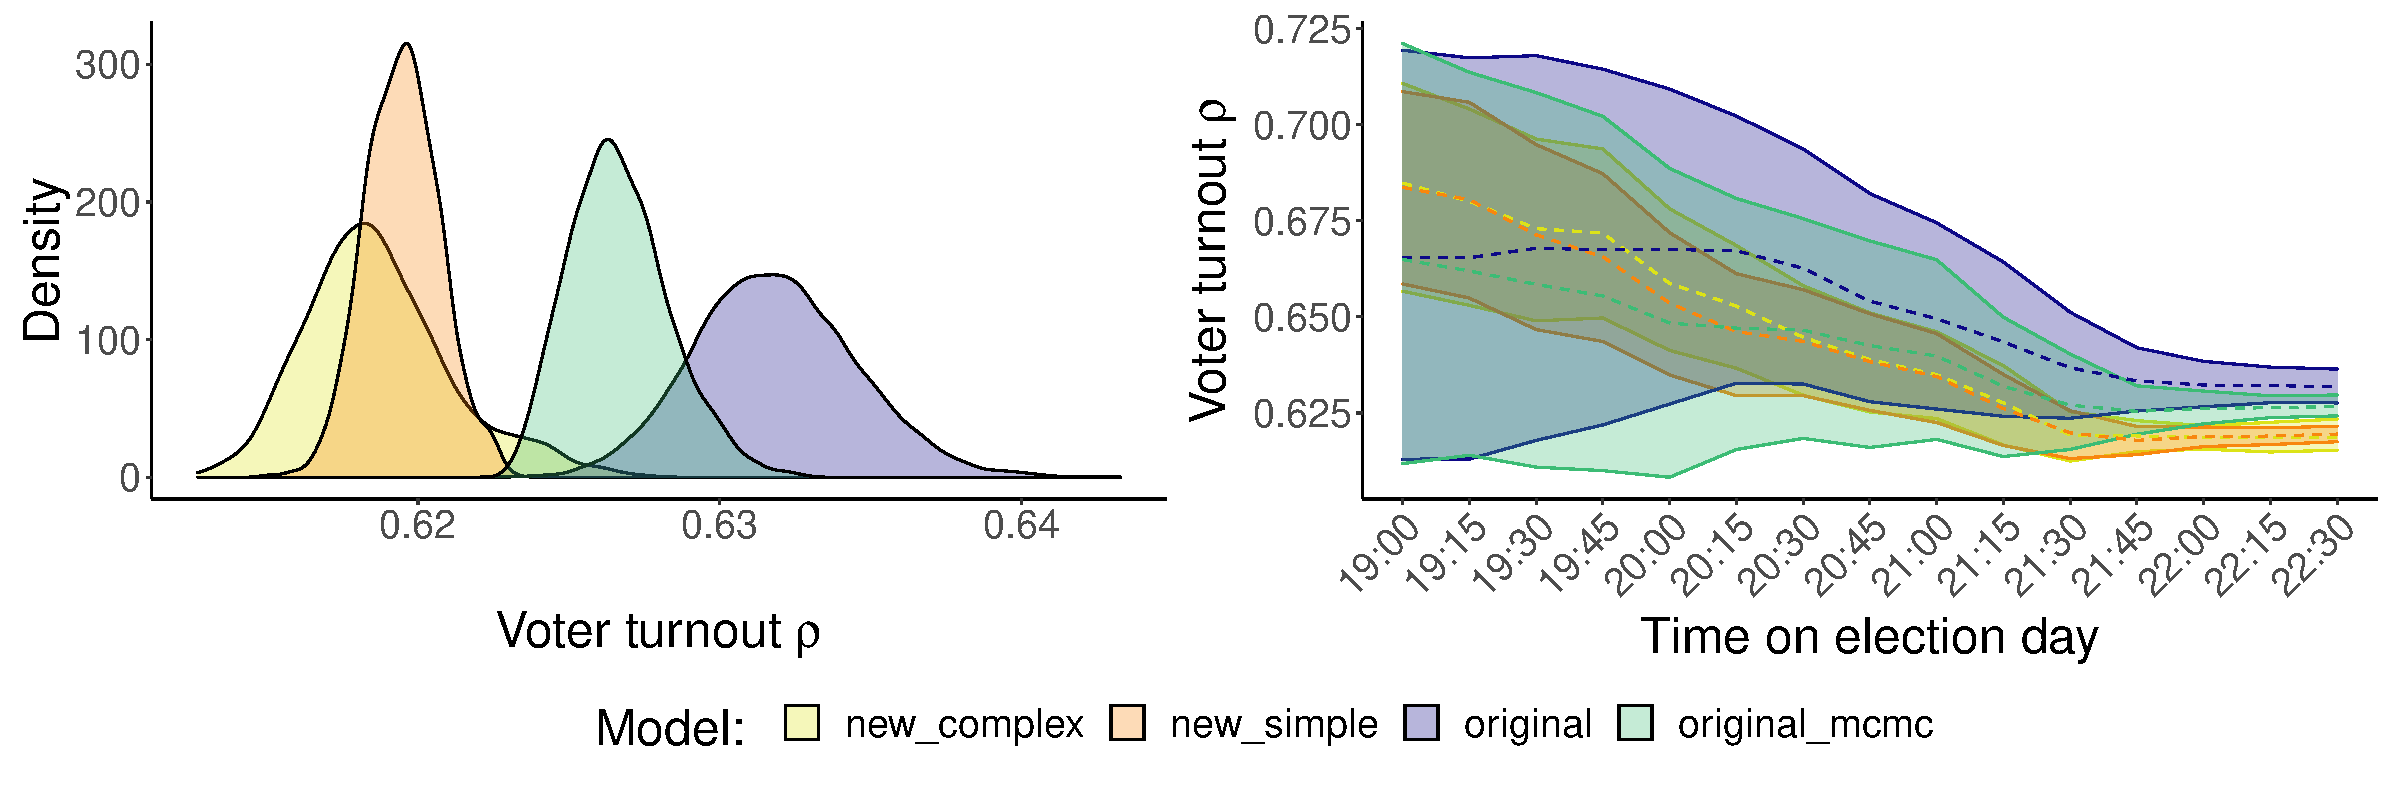
\includegraphics[width=\textwidth]{../fig/part.pdf}
  \caption{The left panel shows the posterior distribution of the voter turnout at 22:30pm, with models by color. The right panel shows the mean and 0.025 and 0.975 quantiles (giving a 95\% posterior credible interval) for different times. \texttt{new\_complex} refers to model 4, \texttt{new\_simple} to model 3, \texttt{original} to model 1, and \texttt{original\_mcmc} to model 2.}
  \label{fig:part}
\end{figure}


Finally, Figure \ref{fig:times} shows the time required to generate samples from each model. Notably, the model with an arbitrary covariance structure requires a lot of time to mix, even for small sample sizes. Interestingly, the new model with a simple covariance structure requires about the same time as the model of \citet{diluvi2018} with an MCMC sampler. However, the former has the advantage of treating the proportions as elements of the simplex, thereby resulting in better estimations of the voter turnout. It should be noted that using MCMC sampling has a clear impact in computation cost: the model with tractable posterior requires $\mcO(1)$ time to train, whereas models 2 and 3 become more expensive as sample size increases.


\begin{figure}[h]
  \centering
  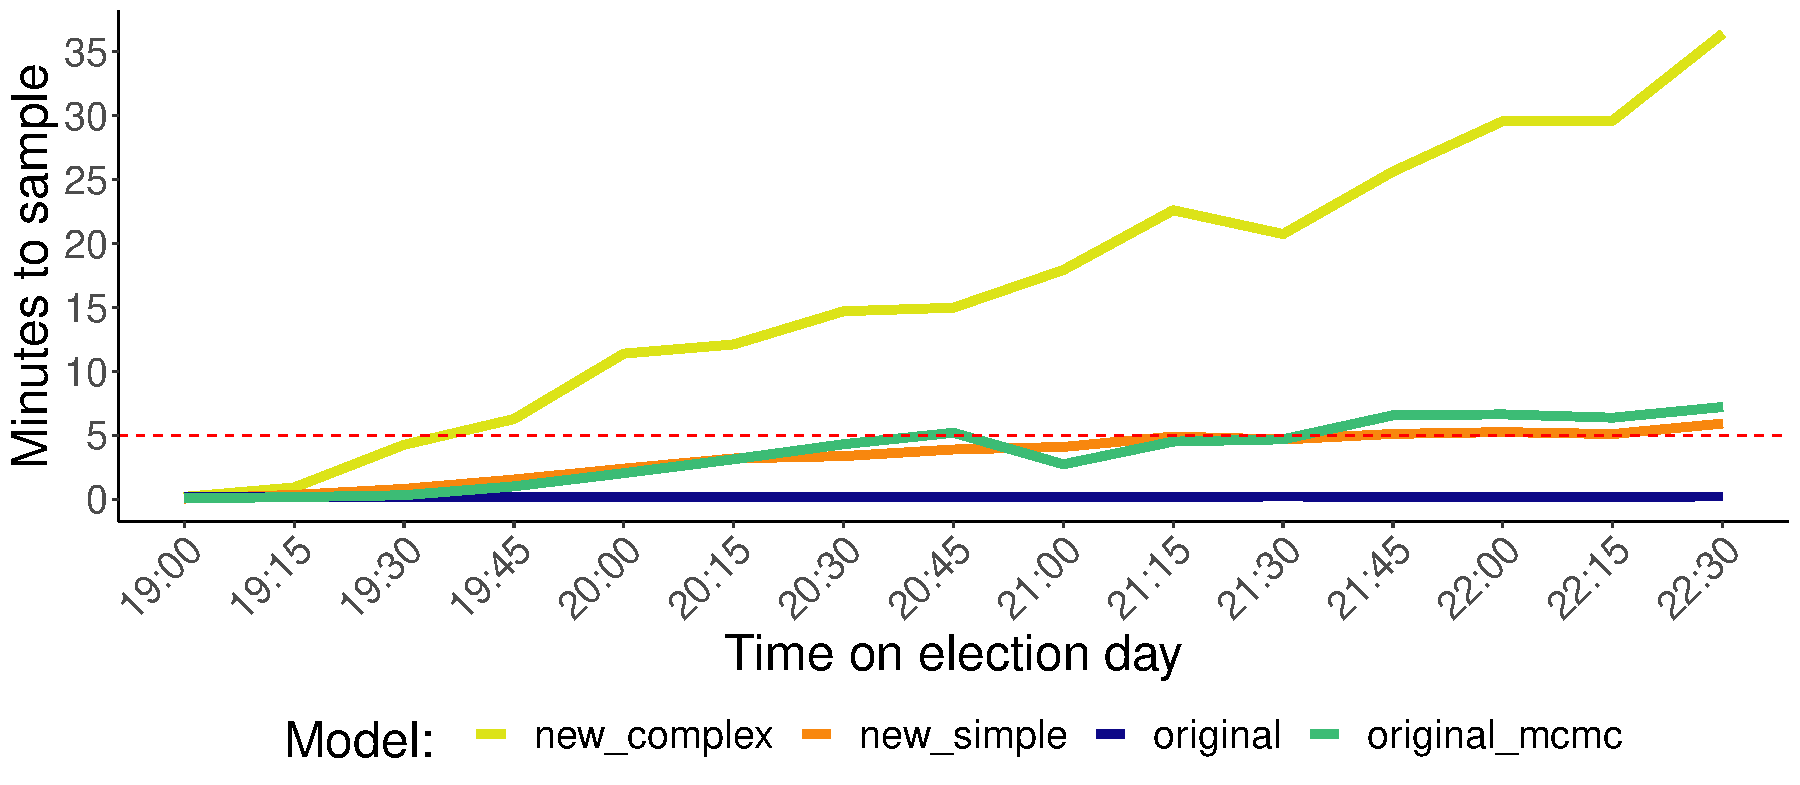
\includegraphics[scale=0.5]{../fig/times.pdf}
  \caption{Time in minutes necessary to generate the posterior samples for each model as a function of time. The red dotted line indicates the 5 minute limit for model training. \texttt{new\_complex} refers to model 4, \texttt{new\_simple} to model 3, \texttt{original} to model 1, and \texttt{original\_mcmc} to model 2.}
  \label{fig:times}
\end{figure}




\section{Conclusion} \label{sec:conclusion}


In this work, we proposed a new general-purpose Bayesian model for estimating the results of Mexican quick counts that \textit{(i)} addresses the known issue of previous Bayesian models overestimating the voter turnout by considering the proportion of votes as an element of the probabilistic simplex; and \textit{(ii)} can be designed to account for arbitrary covariance structures. We also discussed uninformative prior distributions for both the vector of proportions of votes and covariance matrix and developed \textsc{Stan} code to sample from the posterior of the model.
\\

The new model successfully reduces the voter turnout overestimation even if a trivial covariance structure is assumed. In this regard, we also observed that working with a non-trivial covariance structure results in very slow mixing times and no noticeable gains in accuracy (on top of the benefits that result from working on the simplex). A possible avenue for future work would be considering special decompositions of the covariance structure that give more flexibility than the trivial structure but are not as expensive as the arbitrary structure.
\\

Some of the densities in Figures \ref{fig:amlo} and \ref{fig:part} have their masses concentrated in very different parts of $[0, 1]$. It should be noted that it is not easy to compare these densities with the known official results of the election: during election day, polling stations officers report the votes after their first count so as to get information to the quick counts committee as early as possible. However, the officers then do a recount, and some votes are subsequently audited in the week after the election. A fair way to compare the models would be to obtain the results from all polling stations, generate multiple sample according to the sampling design used on election day, and train each model in each sample. It would then be possible to compare the errors of each model. However, to the best of our knowledge such a data base is not publicly available. As for the densities in Figures \ref{fig:amlo} and \ref{fig:part}, we believe the discrepancy might be due to the small number of posterior samples generated.
\\

Another line of research is to design faster schemes for model learning. As seen in Figure \ref{fig:times}, even the models with a simple covariance structure require over 5 minutes to generate posterior samples when the sample size is relatively large. One possibility would be to use sequential Monte Carlo \citep{stewart1992, gordon1993, kitagawa1996} or variational inference \citep{jordan1999, wainwright2008}.




\clearpage
\small
\bibliographystyle{abbrvnat}
\bibliography{../ref}

\end{document}
